\documentclass{article}
\usepackage{color}
\usepackage{listings}
\usepackage{graphicx}
\usepackage{xcolor}
\usepackage{amsmath}
\usepackage{subcaption}
\usepackage{cleveref}

%\pagecolor[rgb]{0,0,0} %black

%\color[rgb]{1,1,1} %grey
\lstset{language=C++,
keywordstyle=\color{blue},
stringstyle=\color{red},
commentstyle=\color{green},
morecomment=[l][\color{magenta}]{\#},
breaklines=true,
breakatwhitespace=true,
numbers=left
}
\title{Assignment \#1}
\author{Asbjørn Bonefeld Preuss\\ Daniel Lomholt Christensen \\ Elie Cueto}
\date{February 2024}
\begin{document}
\maketitle
\section*{Write C++ code that integrates sir for default parameters}
For this C++ code, please see the end of this file
\section*{Plot S, I, R (t)}
In figure \ref{subfig:plot4}, the SIR model was used to simulate a disease spreading through a population of 1000 people. In the model, the recovery took 10 days, The disease had a beta factor of 0.2, meaning the amount of people per day infected, per infected. The simulation ran for 200 days, had only one infected at day 0. The differential equations were evaluated at time steps of 0.1 days.
\begin{figure}
  \centering
  \begin{subfigure}{0.3\textwidth}
    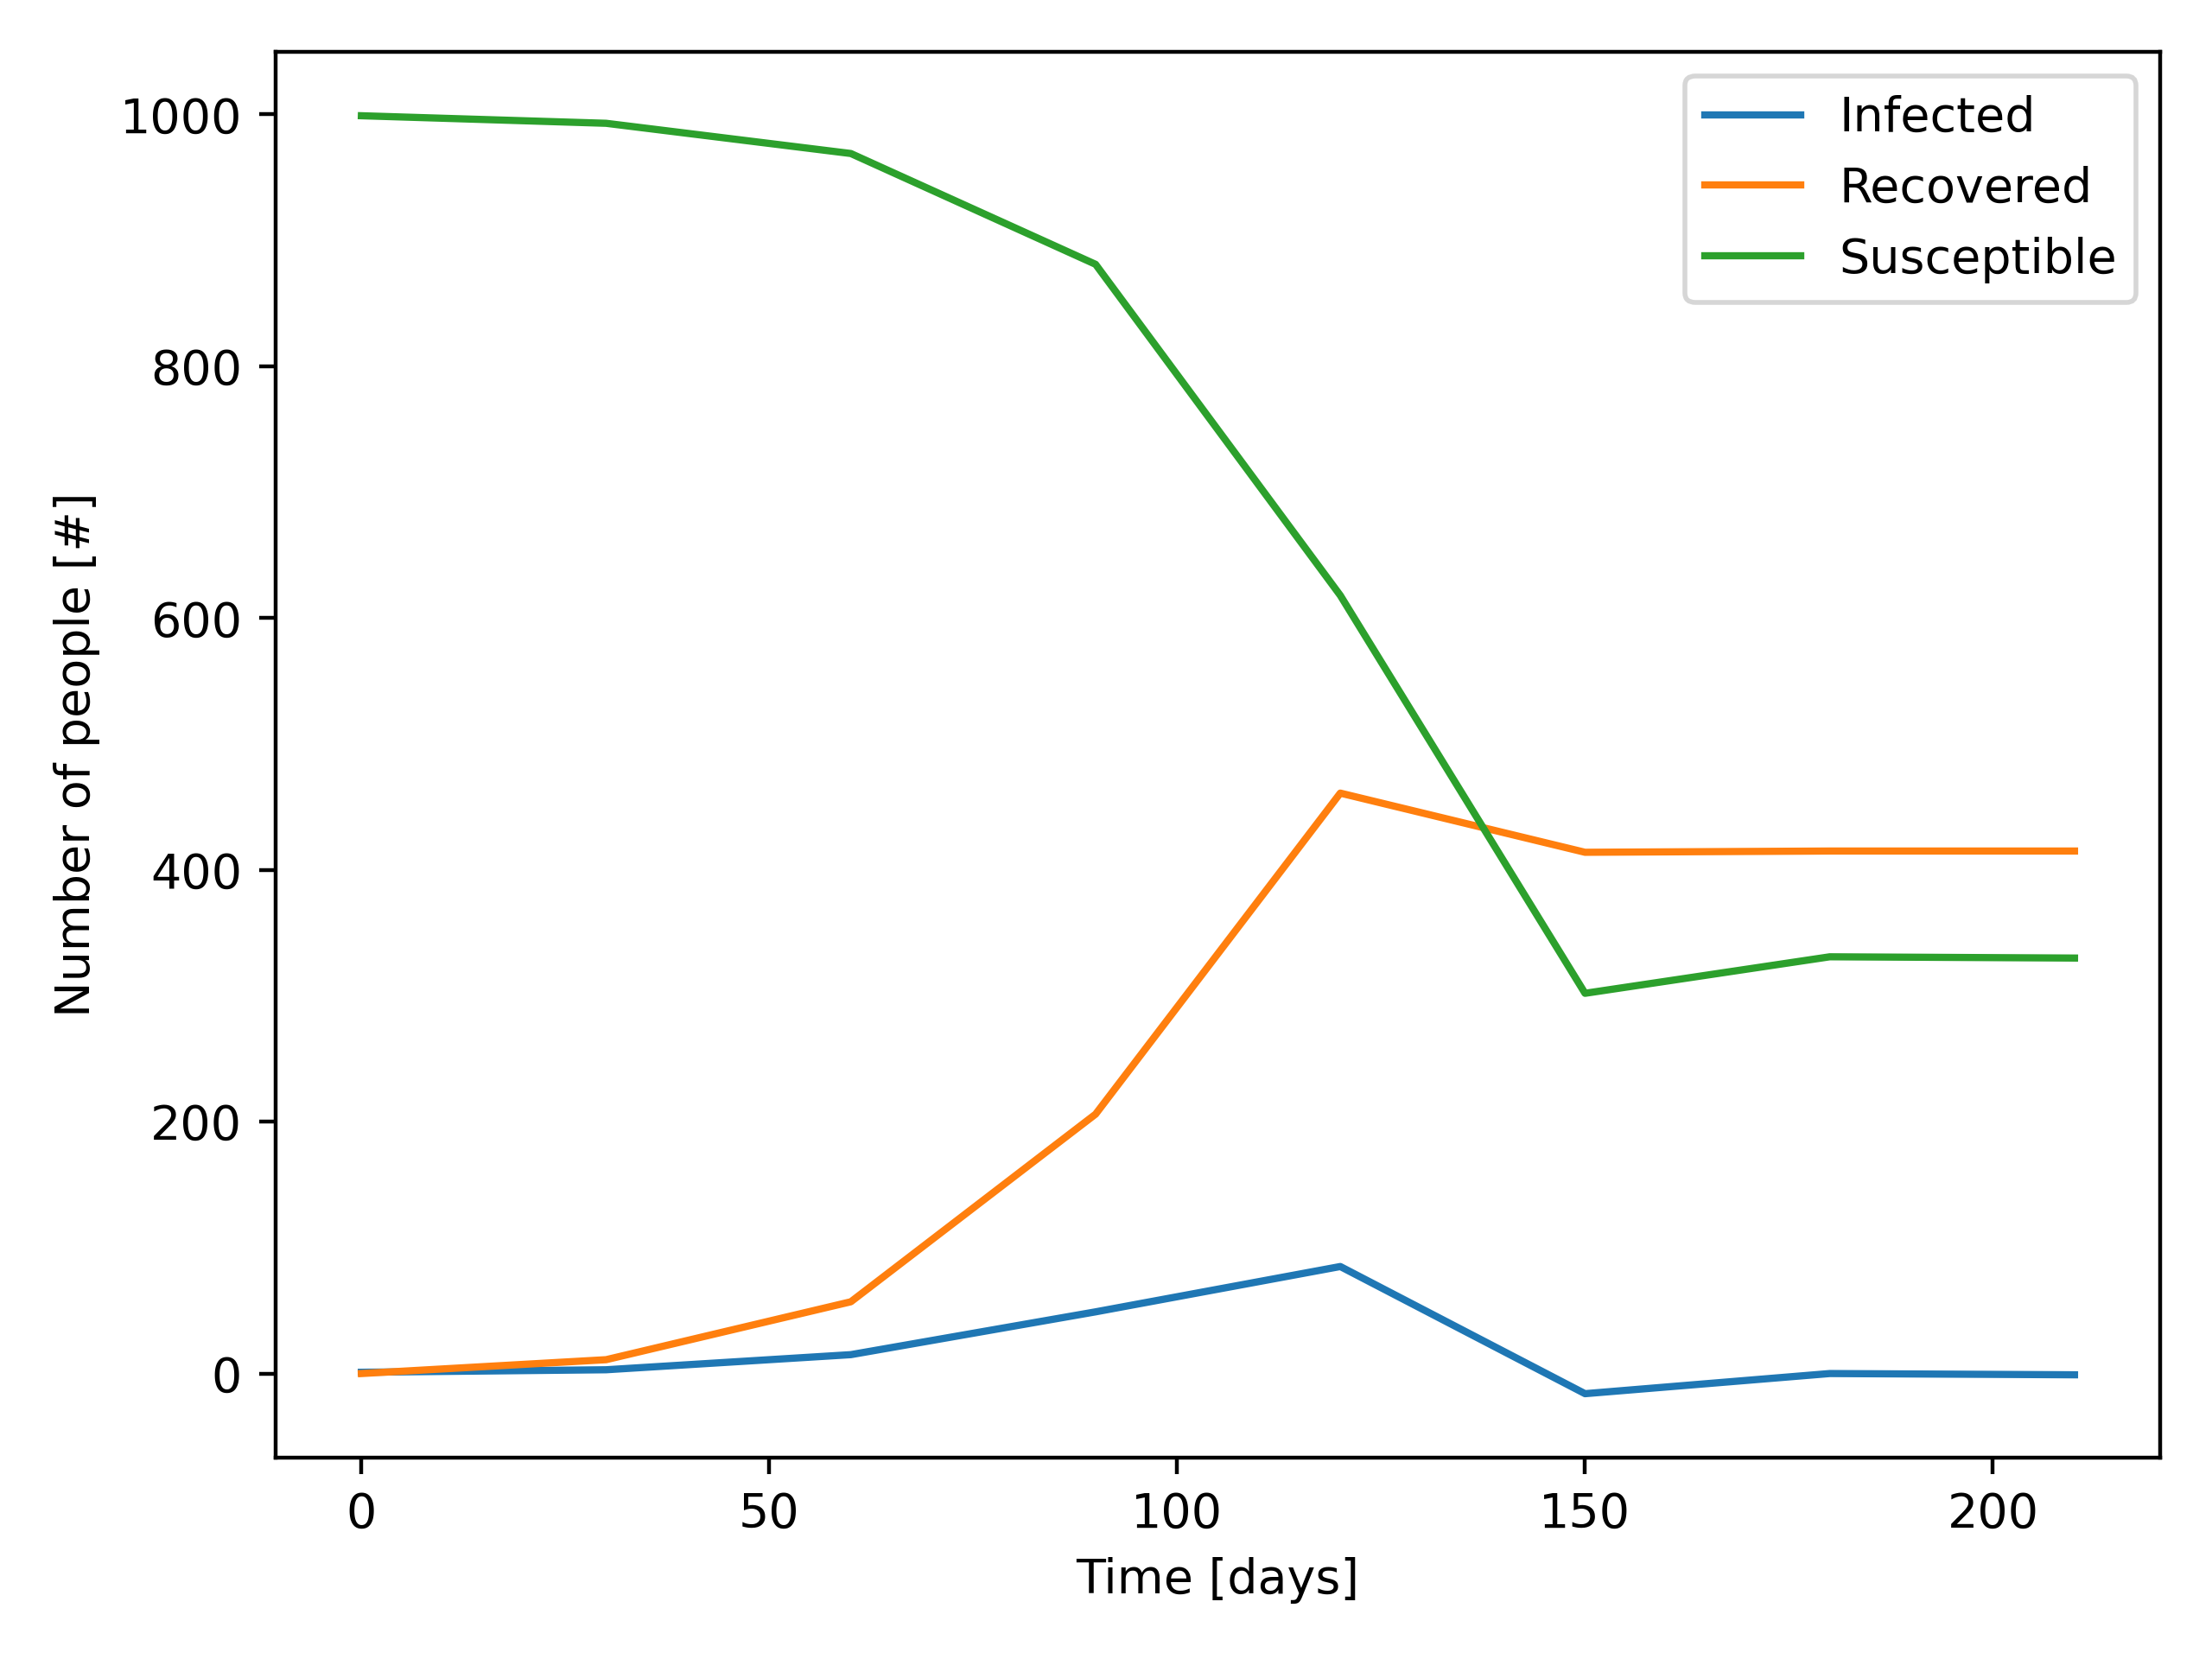
\includegraphics[width=\linewidth]{./Images/SIR_plot_dt30.png}
    \caption{${\rm d}t=30$}
    \label{subfig:plot1}
  \end{subfigure}
  \begin{subfigure}{0.3\textwidth}
    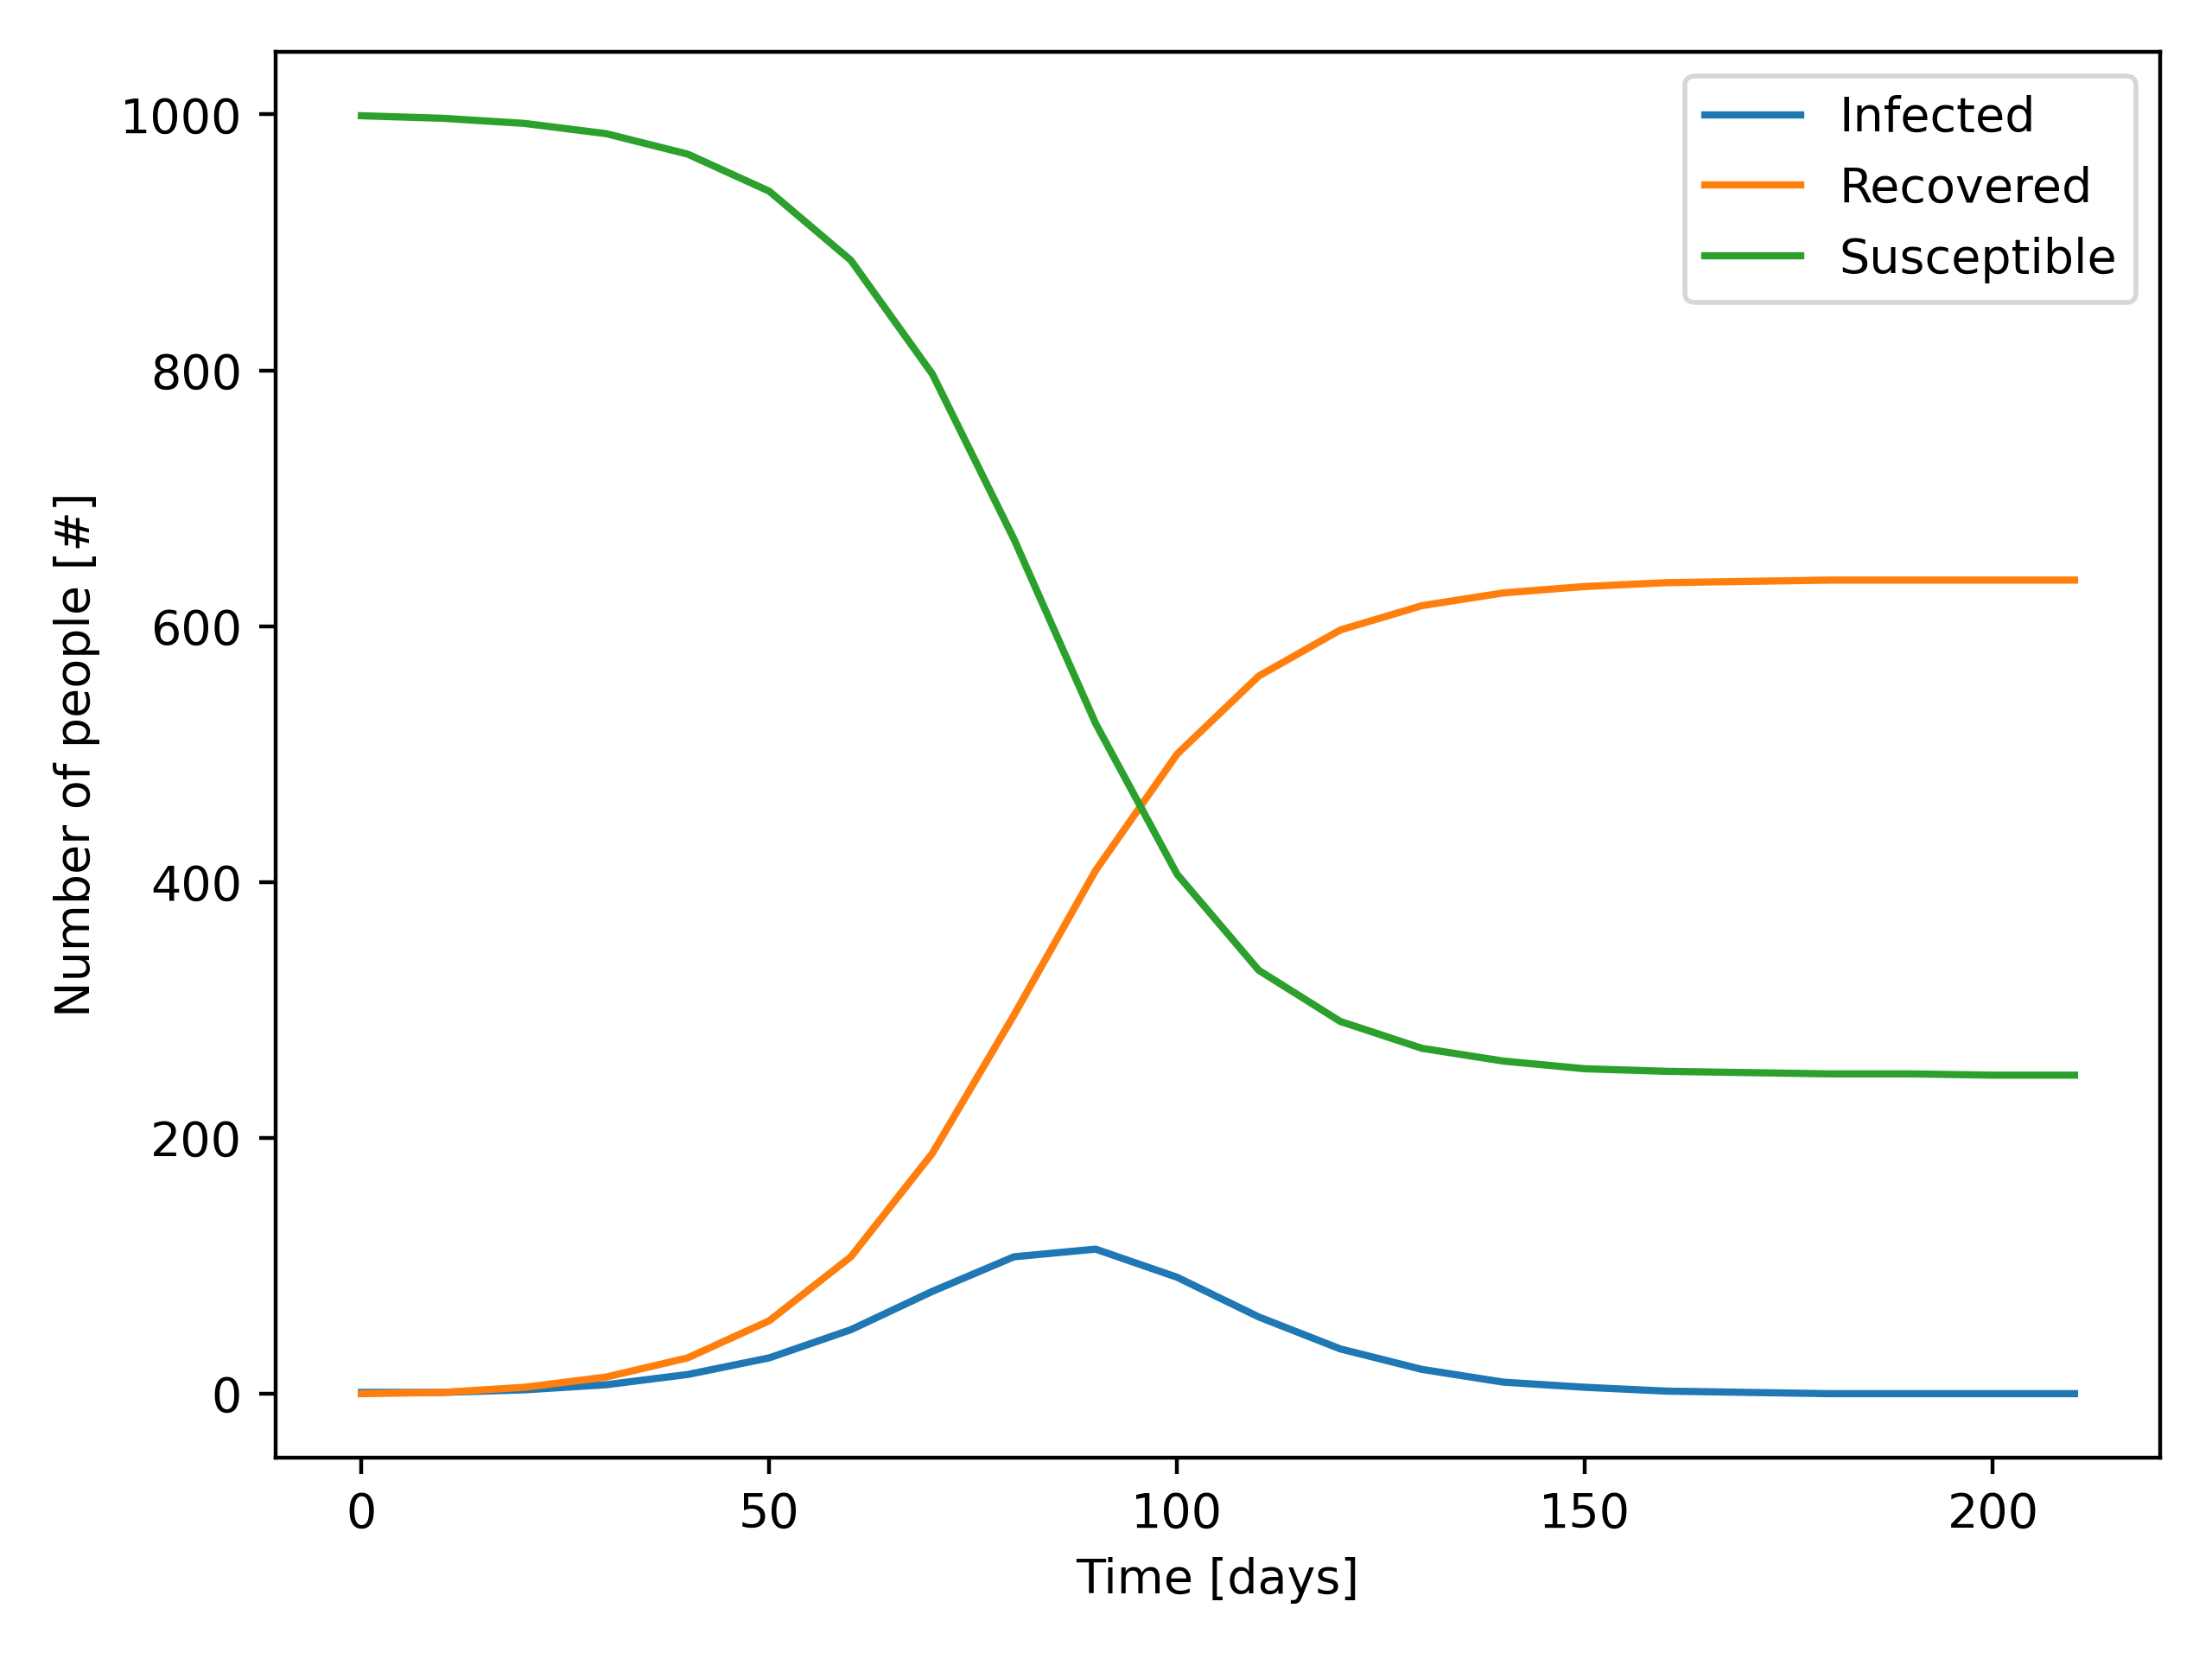
\includegraphics[width=\linewidth]{./Images/SIR_plot_dt10.png}
    \caption{${\rm d}t=10$}
    \label{subfig:plot2}
  \end{subfigure}
  \begin{subfigure}{0.3\textwidth}
    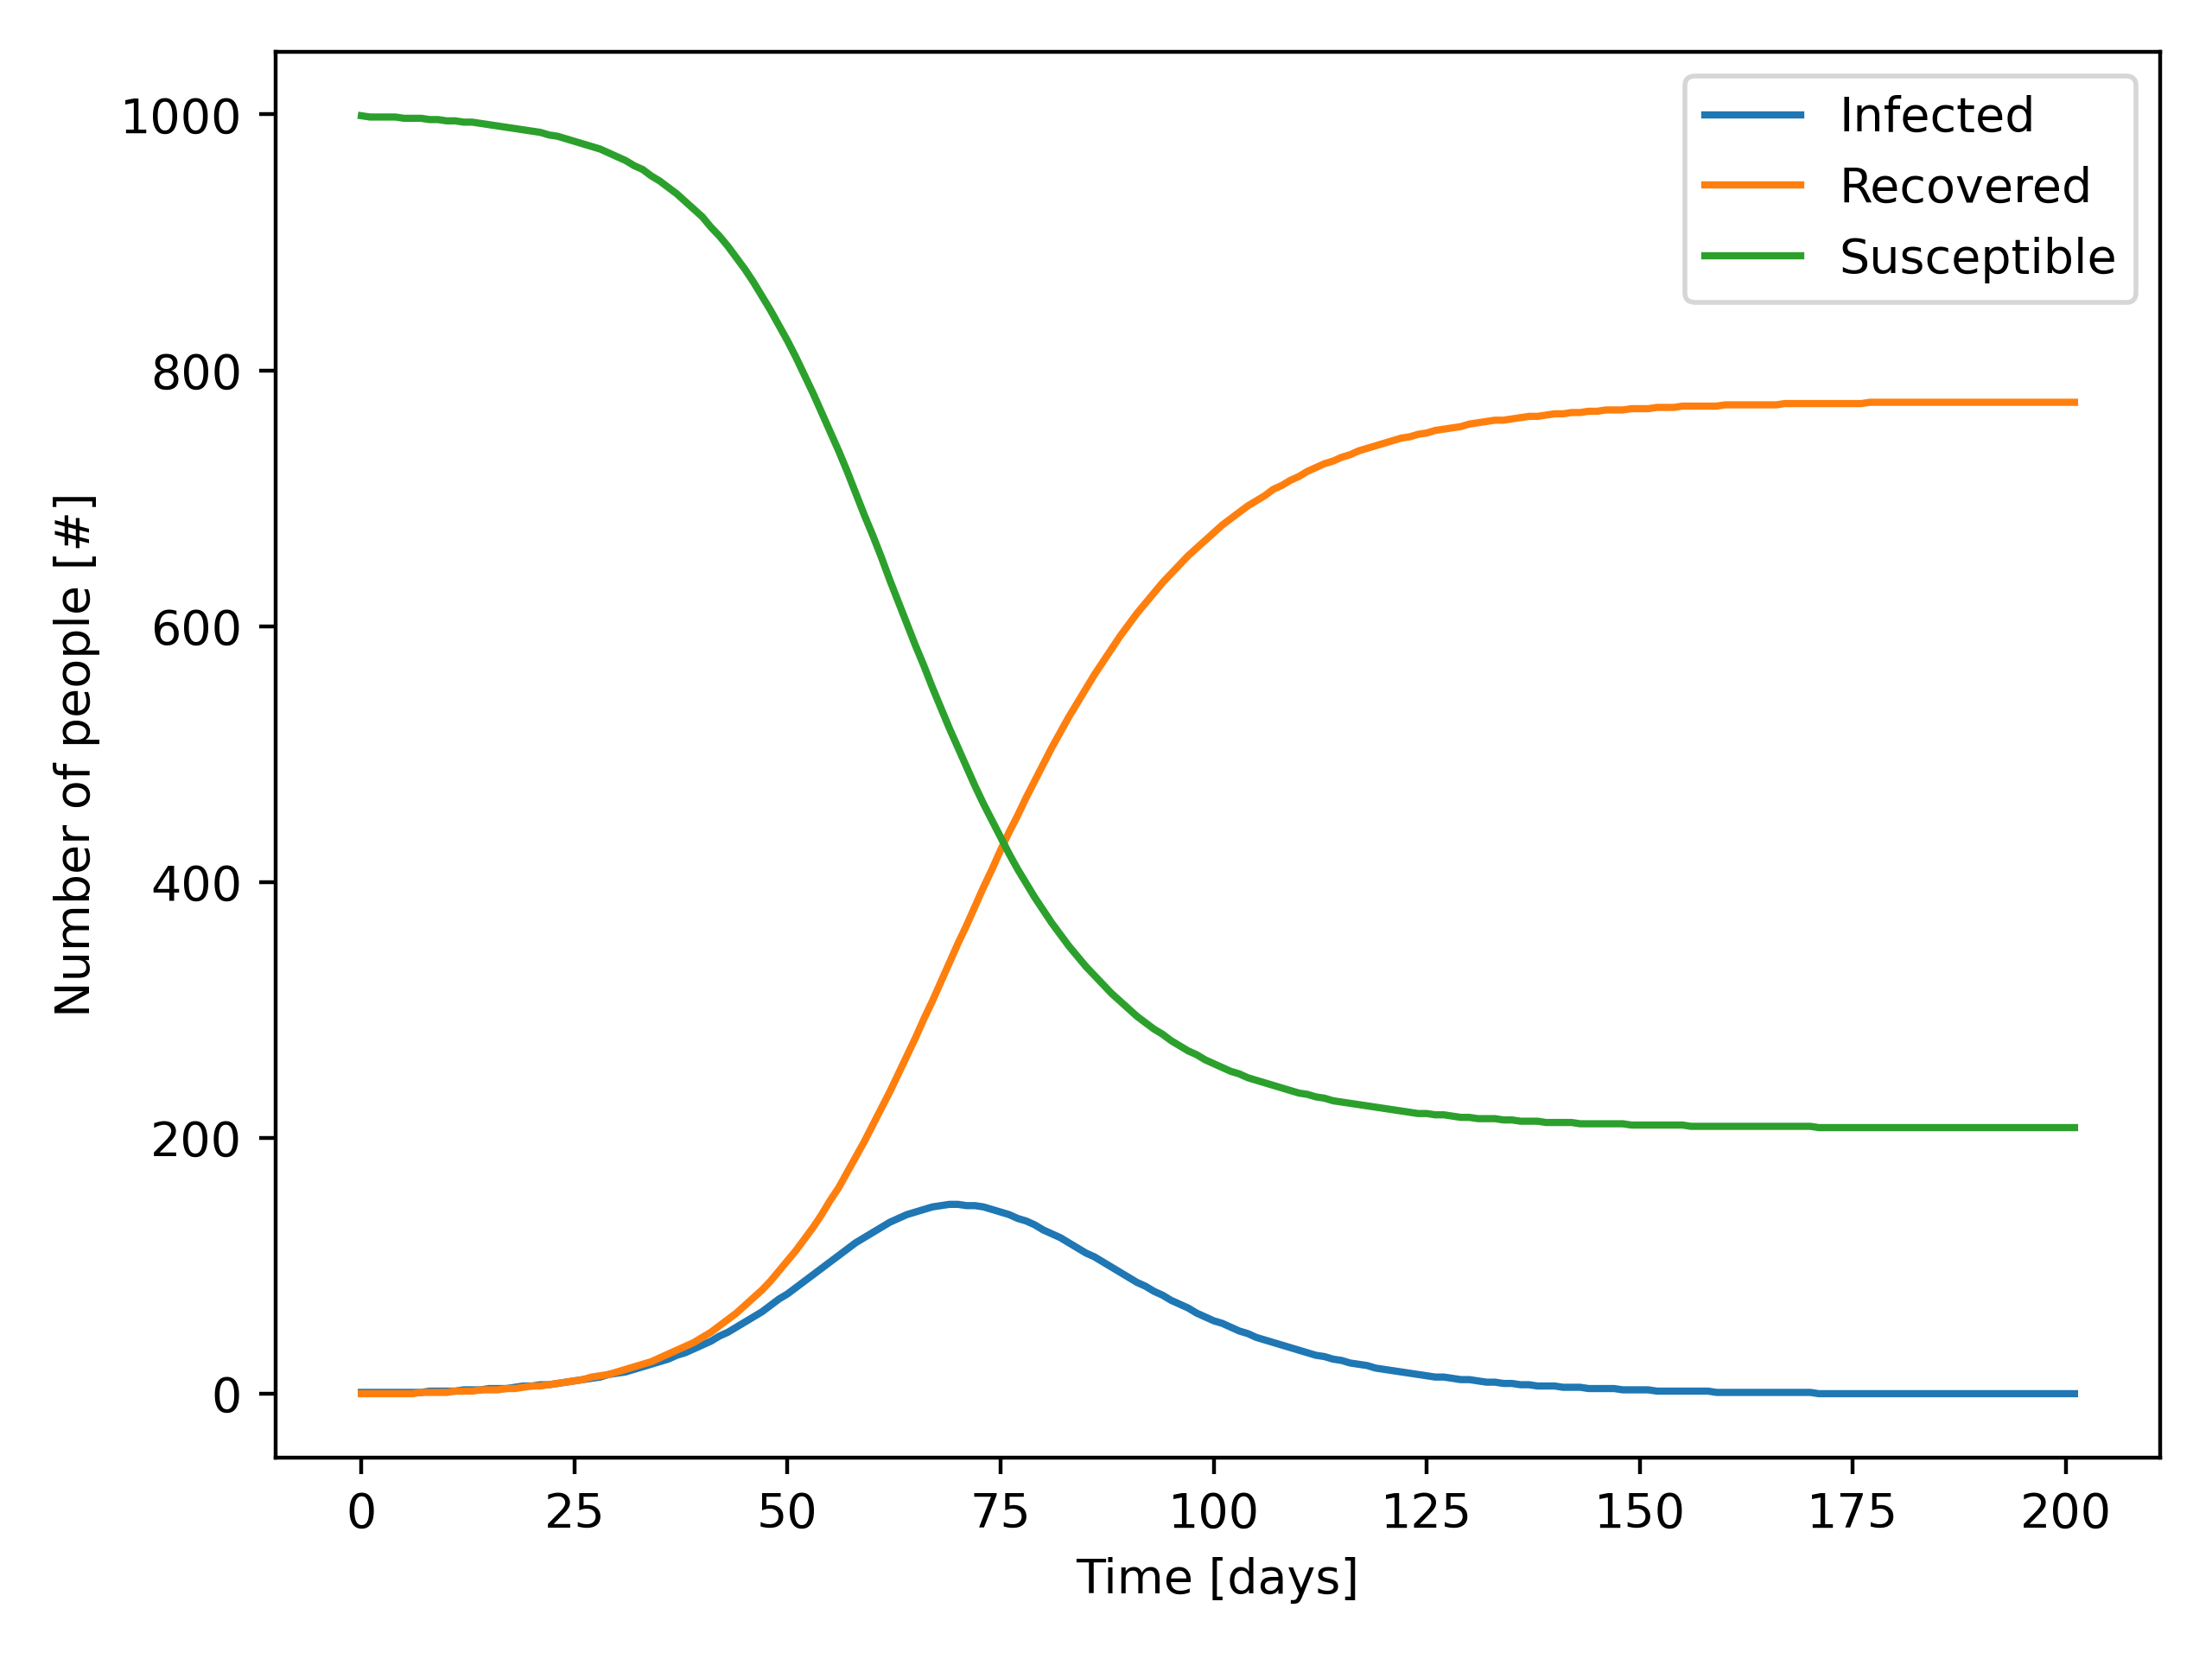
\includegraphics[width=\linewidth]{./Images/SIR_plot_dt1.png}
    \caption{${\rm d}t=1$}
    \label{subfig:plot3}
  \end{subfigure}
  
  \medskip % Add some vertical space between the rows
  
  \begin{subfigure}{0.45\textwidth}
    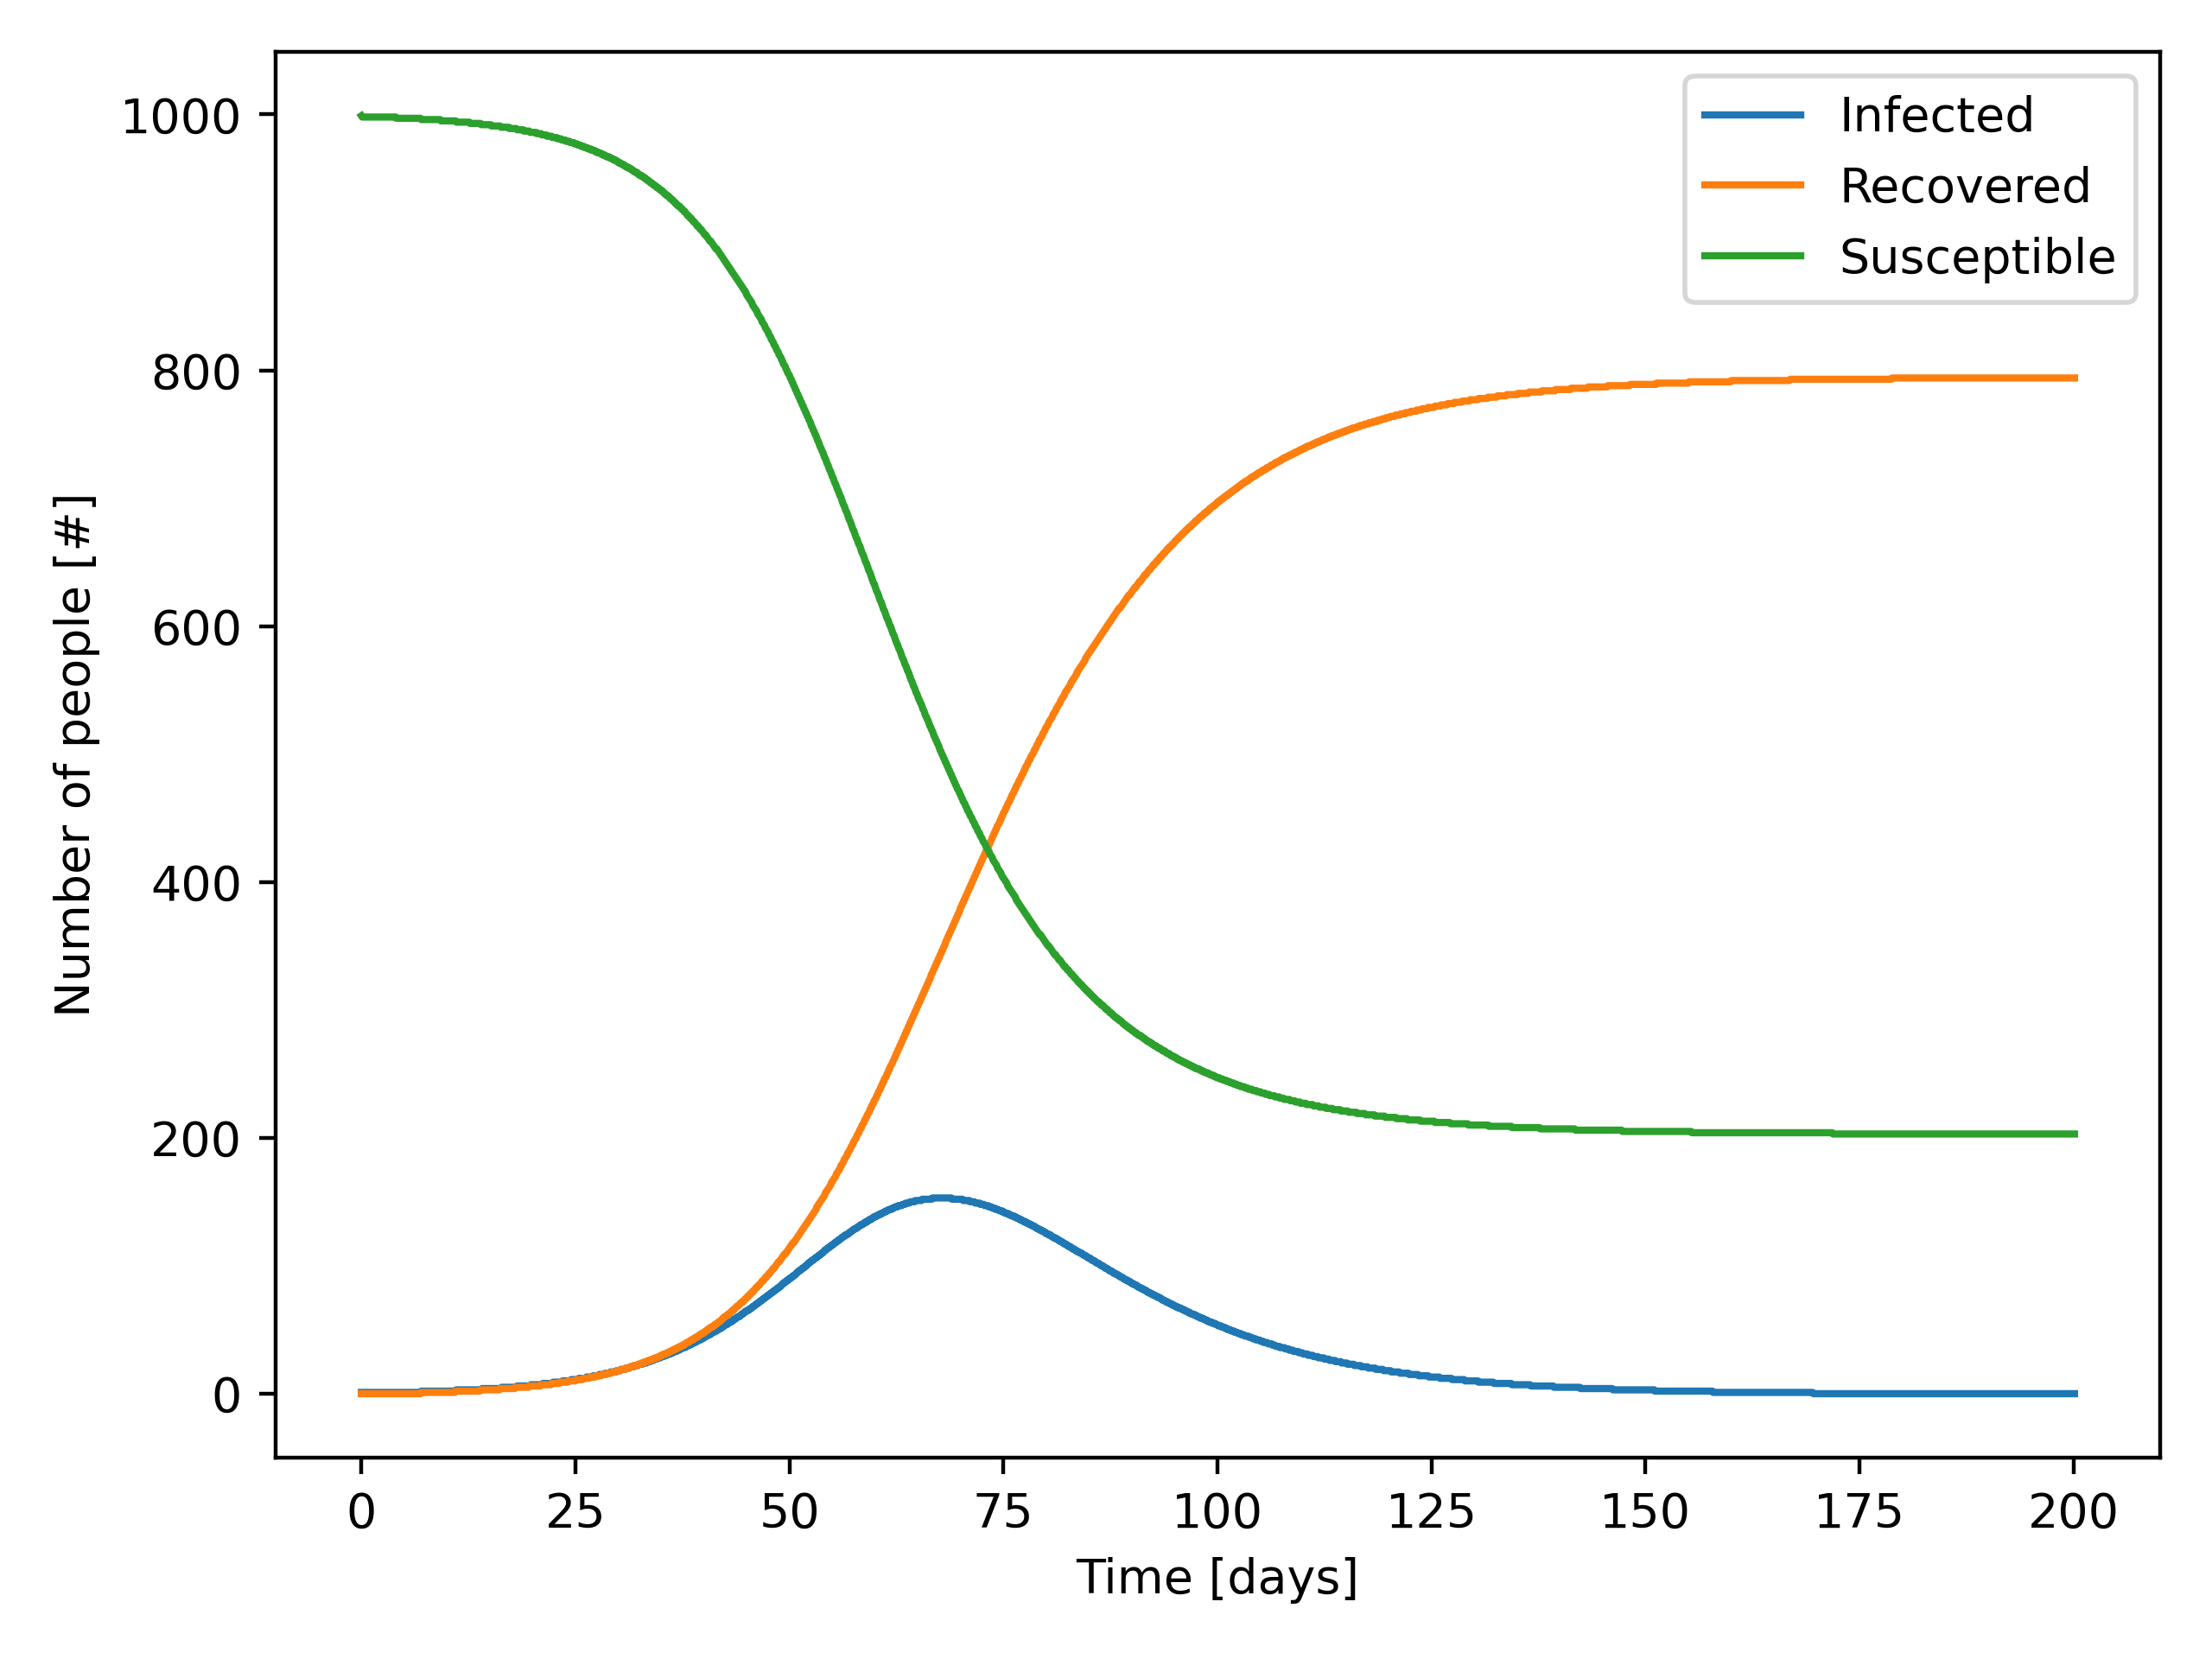
\includegraphics[width=\linewidth]{./Images/SIR_plot_dt0_1.png}
    \caption{${\rm d}t=0.1$}
    \label{subfig:plot4}
  \end{subfigure}
  \begin{subfigure}{0.45\textwidth}
    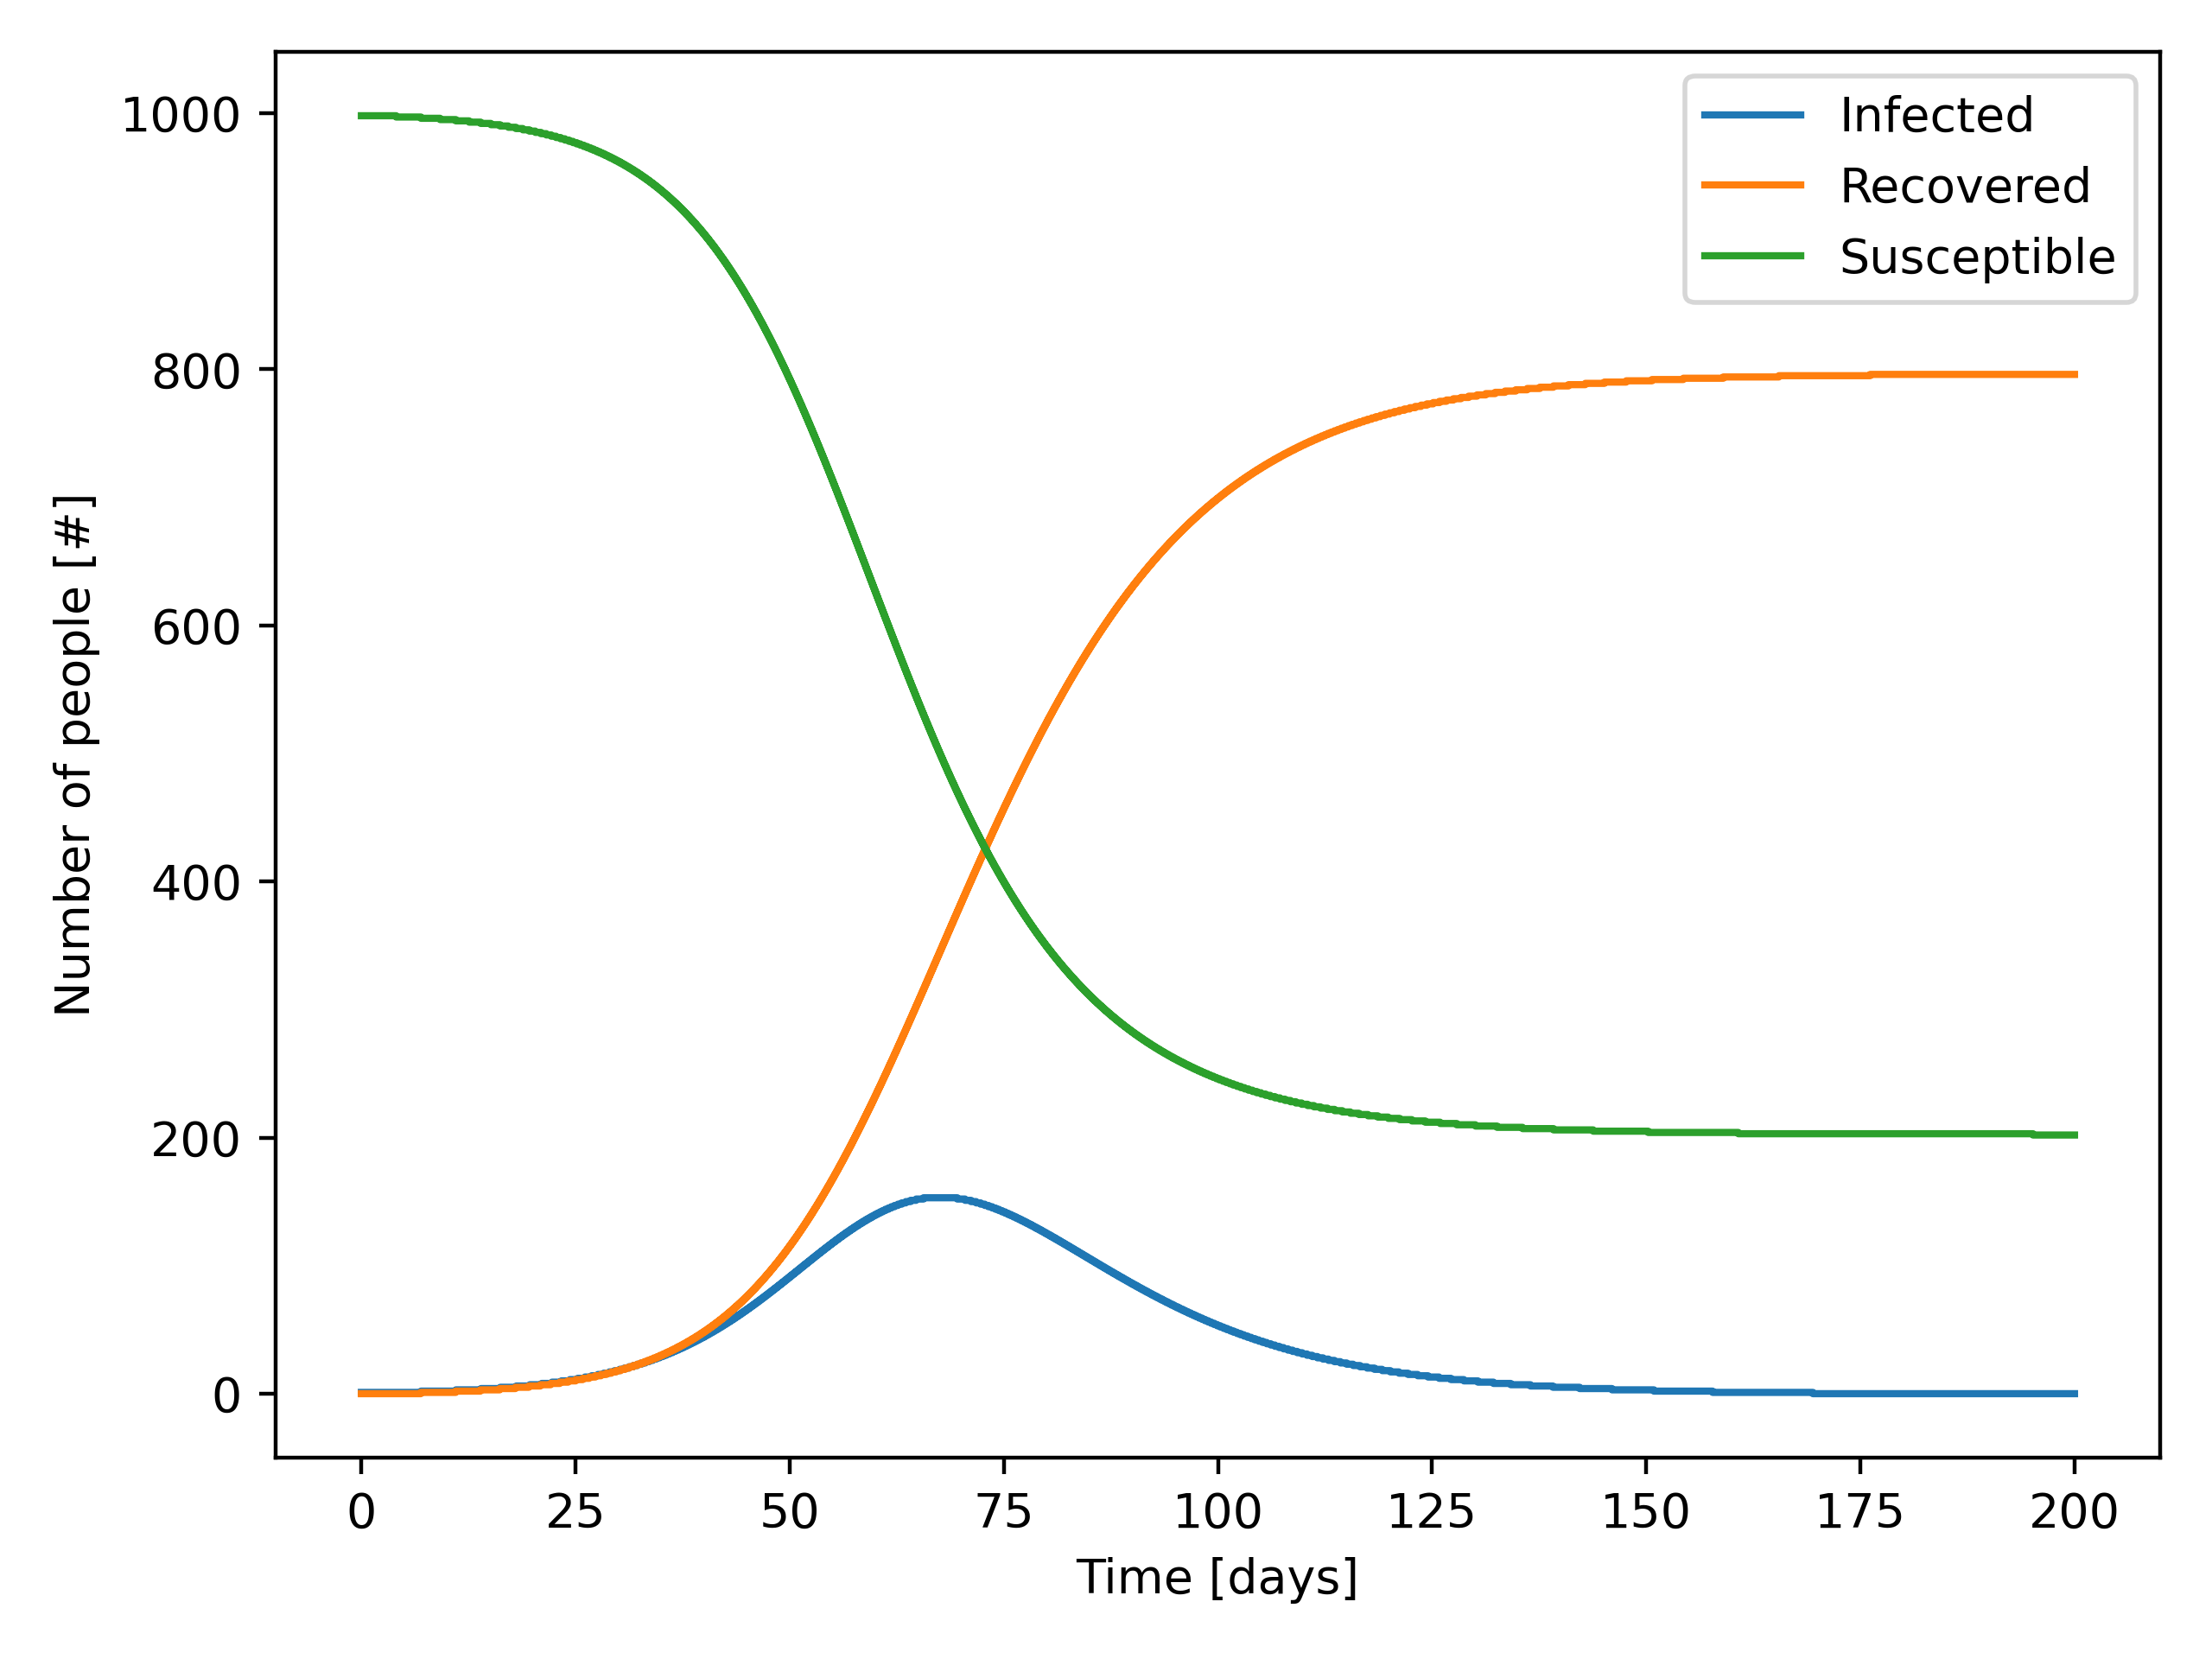
\includegraphics[width=\linewidth]{./Images/SIR_plot_dt0_001.png}
    \caption{${\rm d}t=0.001$}
    \label{subfig:plot5}
  \end{subfigure}
  
  \caption{5 different resolutions for the integration. ${\rm d}t = 0.001, 0.1, 1, 10,$ and $30$. The difference between ${\rm d}t=0.1$ and ${\rm d}t = 0.001$ is almost invisible to the naked eye (and zoom).}
  \label{fig:subplots_two_rows}
\end{figure}
\section*{How many people should be vaccinated to avoid an epidemic?}
The necessary amount of people to vaccinate to avoid an increase in infected people can be found from the differential equations. We want dI to be negative, this means that the recovery rate multiplied by the amount of infected, must be larger than the infected multiplied with the beta factor and the fraction of susceptible people in the population. Therefore it can become a deterministic equation where,
\begin{align}
    \frac{\text{d}I}{dt} &= \beta I \frac{N-I-R}{N} - \gamma I\\
 \gamma I N&=    \beta I (N-I-R) \\
     R &= \frac{\beta(N-I) - \gamma N}{\beta}.
\end{align}

\begin{figure}
    \centering
    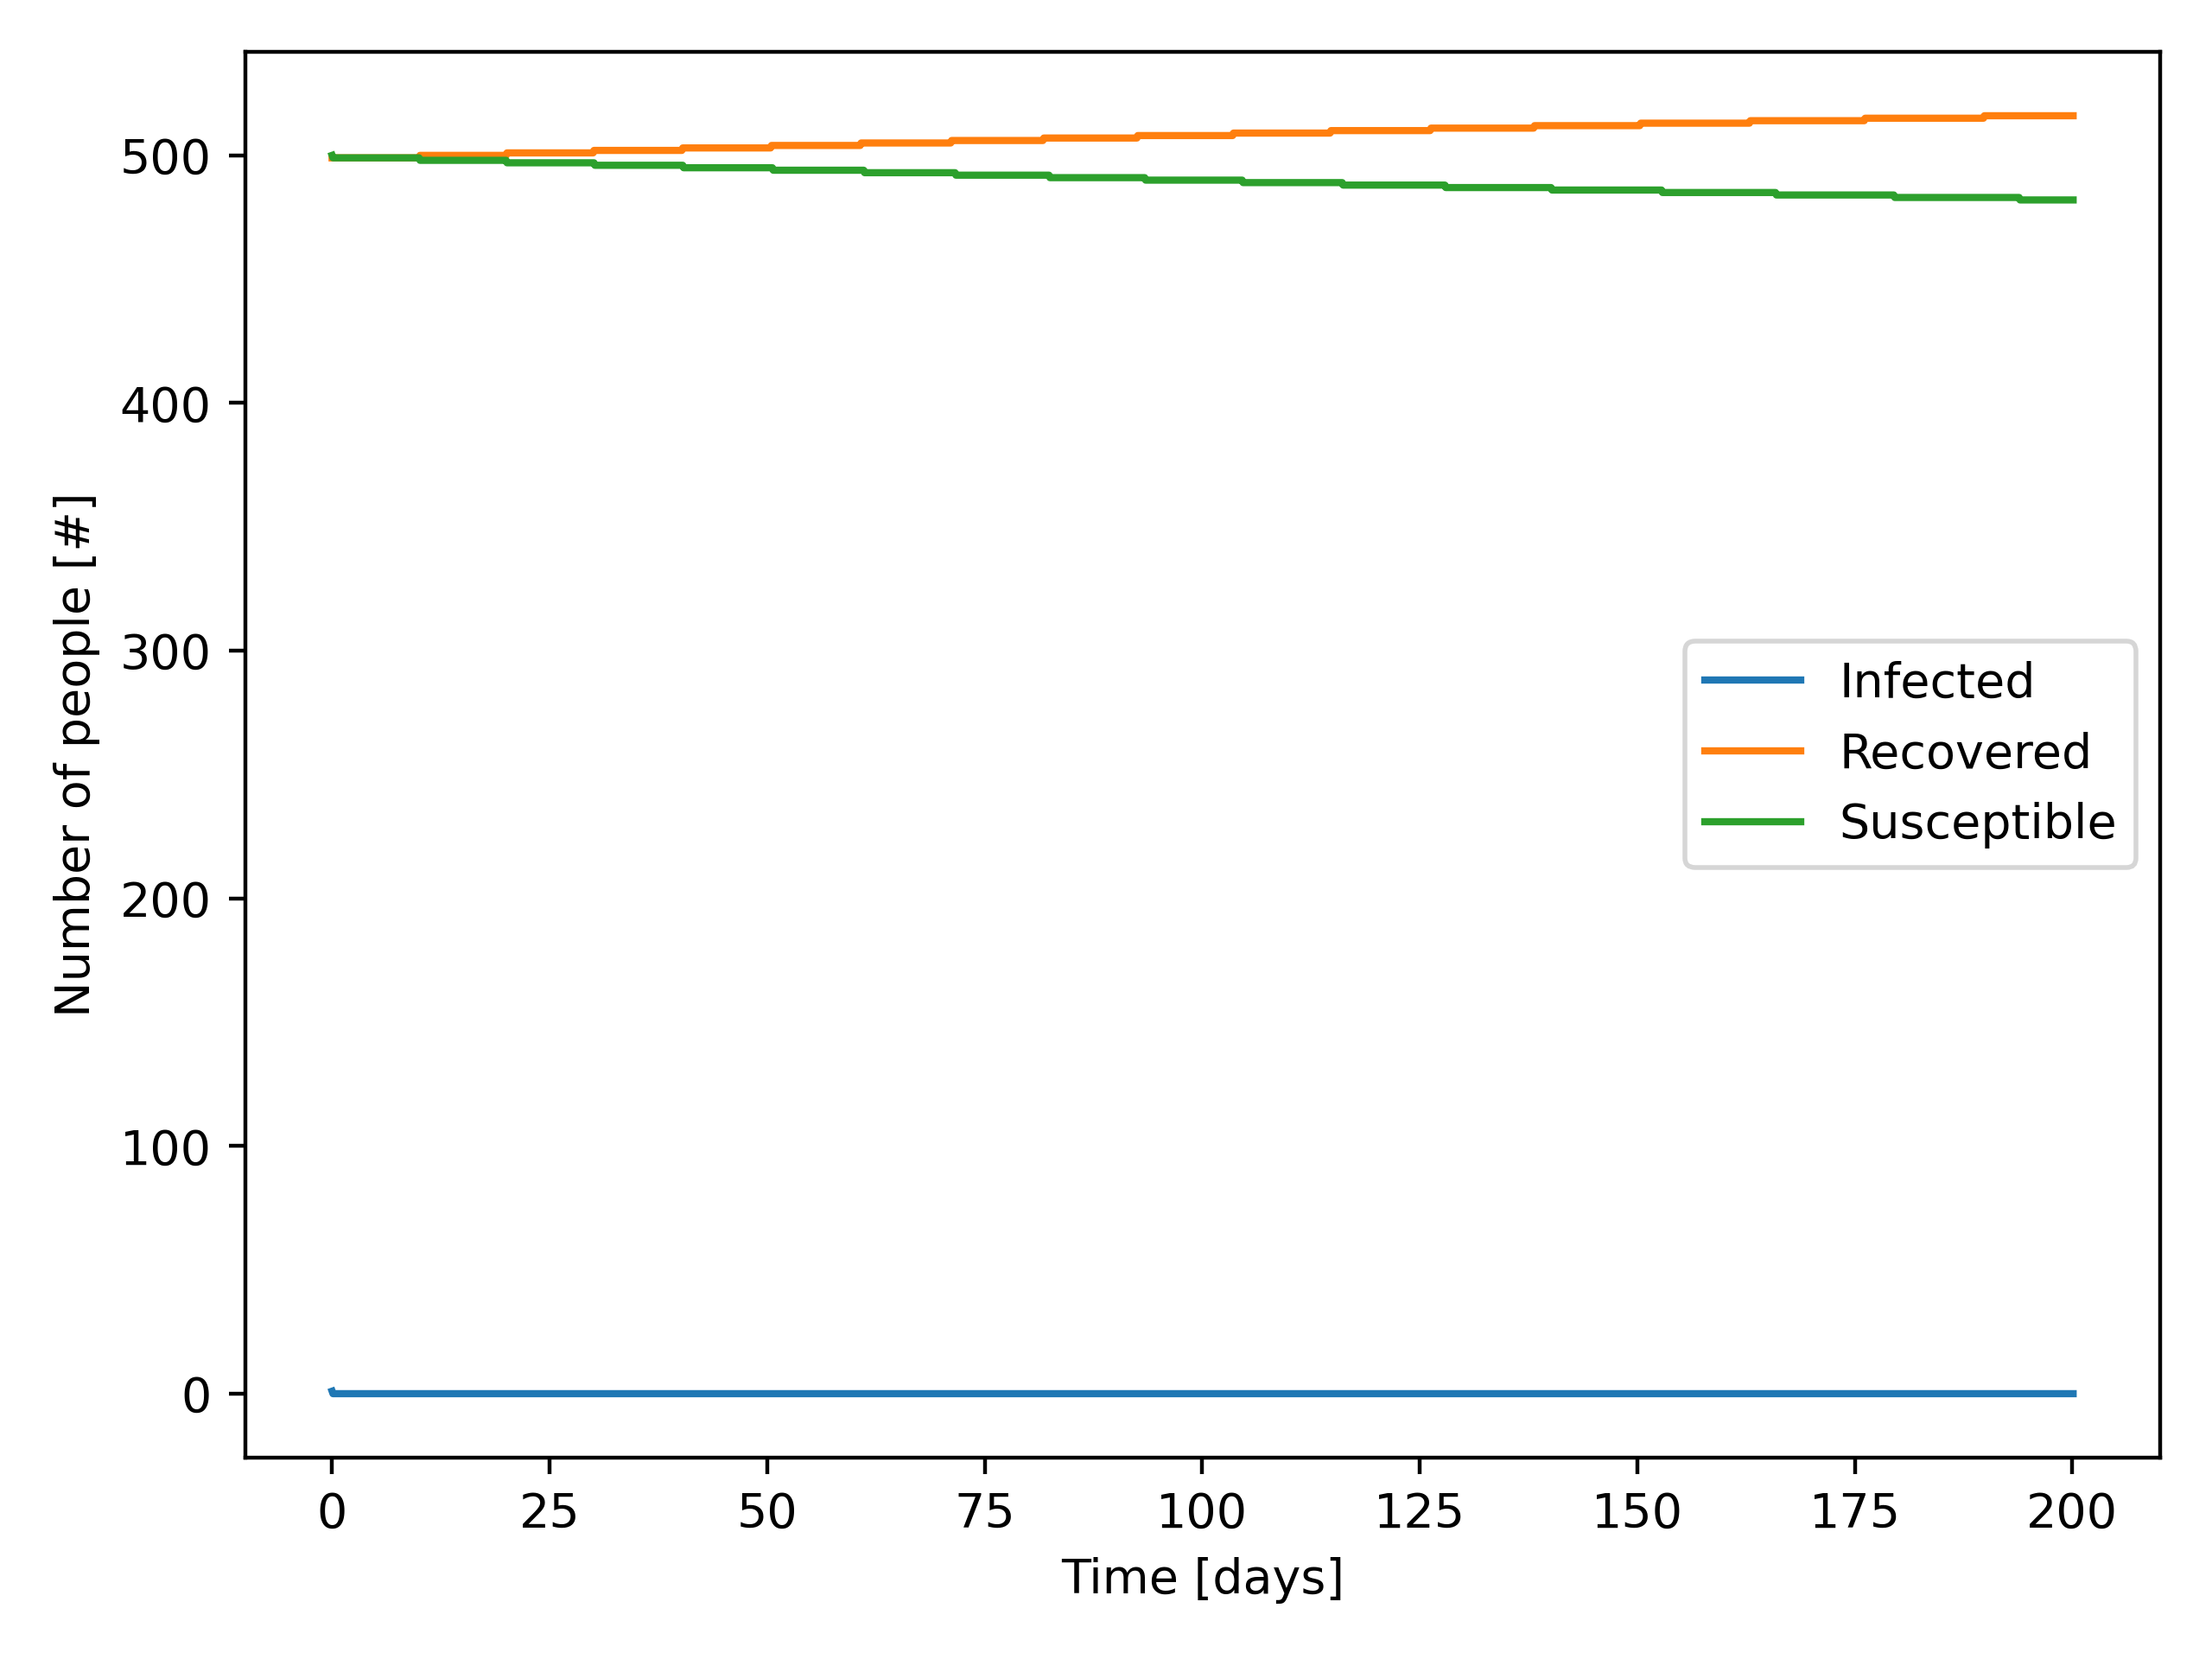
\includegraphics[width=\textwidth]{Assignment_1_SIR/Report/Images/SIR_plot_dt0_1_vacc.png}
    \caption{Results from having 499 out of 1000 people vaccinated from day 0.}
    \label{fig:vacc}
\end{figure}

So the size of the vaccinated population when an epidemic must be avoided should be (in the above example) $(0.2(999)-0.1\cdot 1000)/0.2 = 499$ people or greater. Simulating with 499 people \cref{fig:vacc} vaccinated and one infected yields the expected results except a drift in the amount of recovered/susceptible explained by the floating point amounts of infected people in the code, as $I<1$ does not mean that $I=0$, and so $\frac{\rm{d}R}{\rm{d}t}$ remains greater than $0$ and $R$ slowly increases.

\section*{How big should our time step be?}
In our implementation we use a forward difference euler scheme, which means that we need a relatively small time step, in order to predict the differential equations properly. We have tested this, and found that at time steps above 1 %TODO Find timestep size
day our simulation is not stable anymore, and the results change significantly, and we therefore need a time step below 1 day. As seen in \cref{fig:subplots_two_rows}.

\section*{$\beta$ and $\gamma$ are uncertain estimates of things that are probably not quite constant. How
do you deal with this?}
In our implementation this problem was not dealt with, but it could be dealt with by pseudo randomly changing the $\beta$ and $\gamma$ values between each time step. Our code has the capabilities for this to be implemented with very little effort, as they are passed to the functions, at each time step.

\section*{How do you know your results are correct? You can never be sure, but provide 5 different methods to strengthen the trust in your results.}
The 5 requested methods are written out below:
\begin{enumerate}
    \item We could test edge cases of the parameters, to see what changes they make, to verify that our simulation breaks down, when it should.
    \item We could choose a much smaller time step to strengthen our trust in the solution to the differential equations
    \item We could compare to the known literature to make sure that we produce similar results.
    \item We could compare to reality, to make sure that our equations and simulations describe the world, and not just a nice model.
    \item We could compare results using different compilers for the code, to double check that we get the same results. If different compilers give different results, it suggests that something is wrong somewhere.
\end{enumerate}
\newpage
\section*{Source Code}
\lstinputlisting[language=C++]{../Code/sir.cpp}
\end{document}
